%% draft_sections_4_5.tex — NAACL 2027 SRW fragment (Sections 4--5)
%% \input this file into paper/srw.tex in place of the three % TODO blocks.
%% Figure labels fig:pipeline / fig:al-scaling are placeholders pending the
%% final figure files (blueprint: Fig 1 = pipeline+data flow, Fig 2 = AL
%% scaling curve or label-provenance distribution).

\section{Methodology}
\label{sec:method}

\subsection{System overview}
\label{sec:method:system}

Our deployed system is a two-channel ensemble over Chinese review text
(Figure~\ref{fig:pipeline}). The \emph{student} channel is a
\emph{hfl/chinese-macbert-base} classifier \citep{cui2020macbert}; the
\emph{judge} channel is a small MLP head on frozen
MegatronBERT-1.3B features. Both channels emit class-probability
vectors $P_s$ and $P_j$, blended with fixed weights $1{:}2$:
\begin{equation}
  \mathrm{dep} \;=\; \tfrac{1}{3}\,P_s \;+\; \tfrac{2}{3}\,P_j .
  \label{eq:dep}
\end{equation}
For the three-class task, a \emph{neutral probability correction
module} refines $\mathrm{dep}$. The module is deliberately not an
independent three-way classifier: it estimates only
$P(\mathrm{neutral})$ and leaves the positive/negative split to
$\mathrm{dep}$. Two estimators of $P(\mathrm{neu})$---a frozen-feature
MLP head and a corpus-trained neutral detector---are mixed as
$p_n = 0.6\,P_{\mathrm{neu}}^{\mathrm{head}} +
0.4\,P_{\mathrm{neu}}^{\mathrm{corpus}}$. Writing $r_{+}, r_{-}$ for the
positive/negative masses of $\mathrm{dep}$ renormalized to sum to one, the
corrected distribution and final blend are
\begin{equation}
  \begin{aligned}
    \mathrm{corr} &= \big[(1-p_n)\,r_{+},\; p_n,\; (1-p_n)\,r_{-}\big],\\
    \mathrm{final} &= \frac{\mathrm{dep} + 0.5\,\mathrm{corr}}{1.5}.
  \end{aligned}
  \label{eq:spec}
\end{equation}
We adopt this targeted correction rather than simpler alternatives:
class weighting, decision-threshold adjustment, focal loss, and
class-balanced oversampling were evaluated and rejected
(Appendix~\ref{app:negative}). Its macro-F1 gain over the
uncorrected blend is positive but not statistically significant
(McNemar $p{=}0.65$; bootstrap 95\% CI $[-0.4,+3.8]$pp;
\S\ref{sec:res-ablations}), so we treat the module as a neutral-recall
repair whose benefit must be re-verified on human400
(\S\ref{sec:res-human400}).

A single post-hoc temperature $T{=}0.37$ calibrates the three-class
probabilities; it is fitted by NLL on the same gold-600 OOF
predictions---in-sample calibration---and is argmax-invariant, so it
affects neither accuracy nor macro-F1. For ultra-short slang-only
inputs, an exact-match lexicon guard overrides the ensemble before
inference (verified conflict-free on gold-600). The binary task uses
the same dep-blend without the correction module and a fixed 0.5
decision threshold.

\begin{figure}[t]
\centering
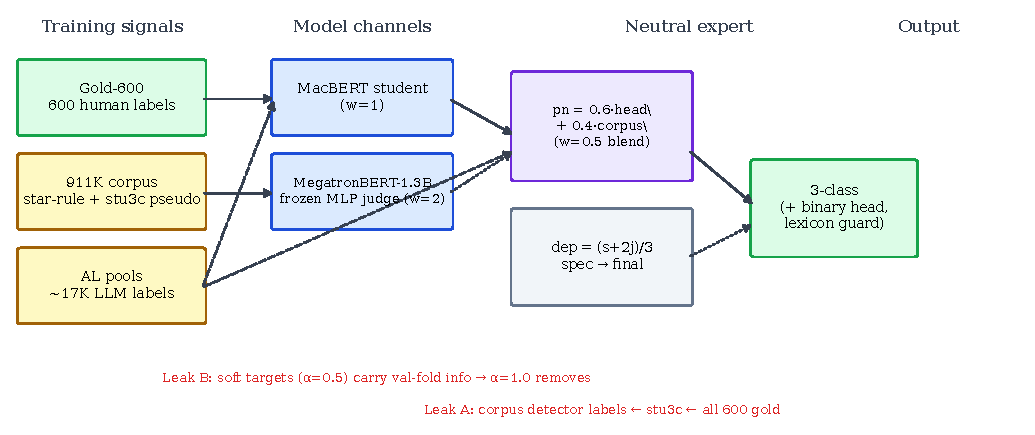
\includegraphics[width=\columnwidth]{fig1_pipeline.pdf}
\caption{Deployed three-class pipeline and its training-signal chain.
Leak~A: the corpus neutral detector's labels descend from stu3c, a
student fit on all 600 gold rows, so its gold predictions carry
whole-set information. Leak~B: distillation soft targets
($\alpha{=}0.5$) are produced by teacher channels whose folds overlap
the student's validation fold. The $\alpha{=}1.0$ ablation removes the
teacher term; the corpus-channel toggle bounds Leak~A.}
\label{fig:pipeline}
\end{figure}

\subsection{Training signal chain}
\label{sec:method:chain}

Labels reach the deployed models through four stages, each of which later
proved relevant to our audit.

\paragraph{Gold seed.} 600 human semantic labels from a single Douban
film page (316 positive / 92 neutral / 192 negative; binary evaluation
on the 508 non-neutral rows) provide hard and soft targets for the
first students and judges.

\paragraph{Distillation objective.} The gold-trained students and the
frozen-feature judge heads are optimized with a mixed hard/soft
objective \citep{hinton2015distilling} rather than plain
cross-entropy: for a training row $i$ with hard label $y_i$ and
teacher probability vector $q_i$ (the deployed teacher ensemble's
stored out-of-fold prediction for that row), the per-sample loss is
{\small
\begin{equation}
  \begin{aligned}
  \ell_i = {}& \alpha\,\mathrm{CE}(z_i, y_i) \\
             & +\; (1-\alpha)\,\tau^{2}\,
  \mathrm{KL}\!\Big(\mathrm{softmax}\big(q_i/\tau\big)\,\Big\|\,
  \mathrm{softmax}\big(z_i/\tau\big)\Big),
  \end{aligned}
  \label{eq:kd}
\end{equation}
}
where $z_i$ are the student's logits, $\mathrm{CE}$ is (optionally
class-weighted) cross-entropy, and the second term is standard
temperature-scaled distillation: both $q_i$ and $z_i$ are divided by
$\tau{=}2$ before the softmax, and the teacher$\,\|\,$student KL
divergence summed over classes is rescaled by $\tau^{2}$. Crucially,
$\alpha$ weights the \emph{hard}-label term, not the teacher term:
$\alpha{=}0.5$ gives hard labels and teacher soft targets equal
weight, while $\alpha{=}1.0$ sets the teacher weight to exactly zero
and recovers pure hard-label training (the same objective trains the
MLP judge heads). Teacher probabilities are fixed per-row vectors
from the deployed teacher ensembles, and teacher and student share
the same 5-fold partition, so the KD term on a student's training
rows is not independent of its validation fold (Leak~B,
\S\ref{sec:audit}); the $\alpha{=}1.0$ ablation removes the teacher
term entirely while holding folds, hyperparameters, and fusion
weights fixed.

\paragraph{Pseudo-label pools.} Following classical self-training and
pseudo-labeling practice \citep{lee2013pseudo,xie2020selftraining}, a
3-class student re-scores all 910{,}998 corpus rows under a
weak-supervision framework \citep{ratner2017snorkel}; the confident
pool ($\mathrm{conf}{\ge}0.7$, 271{,}905 rows) is sampled under
per-class caps into 115K--195K-row training subsets for full-fit
corpus-trained models. Binary pools use $\mathrm{conf}{\ge}0.8$;
star-rating-derived label variants serve as ablations.

\paragraph{Corpus-trained models.} Full-fit MacBERT students and
frozen-feature MLP heads are trained on these pseudo-label pools,
including the deployed neutral corpus detector.

\paragraph{Active learning and SFT mixes.} Margin-band
($[0.15,0.70)$) and cross-student disagreement mining select 17{,}000
mutually disjoint corpus rows, labeled by LLM teachers (DeepSeek-V4.1-Flash
primary; Qwen3-4B and hybrid variants as comparisons) in rounds from
1K to 17K labels. A per-fold SFT student is trained on gold$+$AL
labels and fused with the deployed ensemble at weight $w_{\mathrm{SFT}}$
selected by 5-fold cross-validation.

\subsection{Audit methodology}
\label{sec:audit}

Alongside the system we contribute a source-aware evaluation
protocol, distinguishing three levels of evaluation independence---
\emph{per-row fold isolation}, \emph{upstream signal isolation}, and
\emph{selection independence}---of which our headline score satisfied
only the first, up to eight exact-duplicate gold-600 texts that can
cross stratified folds (Appendix~\ref{app:audit} gives the taxonomy).
Two leak mechanisms violate upstream signal isolation.
\textbf{Leak~A} (transitive pseudo-label): a channel's training labels
are outputs of a model fit on 100\% of the evaluation labels---the
chain gold$\to$stu3c$\to$911K pseudo-labels$\to$corpus detector places
gold information inside the deployed neutral channel at $\approx$13\%
effective weight. \textbf{Leak~B} (second-order teacher): per-fold
soft distillation targets (Eq.~\ref{eq:kd}) are emitted by teachers
whose own folds overlap the student's validation fold, so at
$\alpha{=}0.5$ the teacher-KD term carries half the loss weight and
half the distillation signal is second-order. Both are invisible to
standard OOF reporting because the CV machinery itself is correct.

Our \emph{leak-isolation protocol} reruns all distilled channels with
$\alpha{=}1.0$ (pure hard-label cross-entropy) holding folds,
hyperparameters, and fusion weights fixed, and toggles the corpus
channel on/off. A \emph{row-level cid audit} intersects every
evaluation set's comment IDs with each corpus-derived model's training
manifest, reporting per-model and union overlap plus near-duplicates.
A \emph{selection-bias accounting} enumerates the full candidate pool
(26 mixtures, $\approx$73 SFT runs), reports every number as a maximum
over it, and distinguishes cross-fit from oracle selection
\citep{dror2018hitchhiker}. All OOD numbers are reported \emph{split
by annotation provenance}.

\section{Experimental Setup}
\label{sec:setup}

\paragraph{Evaluation sets.} Table~1 (\S\ref{sec:data}) inventories all
label sources; here we fix the \emph{role} of each set under the audit.
\textbf{gold-600 OOF} was never used for Stage-2 OOD model selection,
but deployed v3's configuration and fusion weights were tuned on
gold-600 itself, so its OOF estimates are not fully selection-
independent (frozen tuned weights, Leak~A/B bounded by the
$\alpha{=}1.0$ ablation, eight exact-duplicate texts able to cross
folds); corrected estimates therefore also rerun all distilled
channels on the deduplicated \textbf{gold-592} set under identical
ungrouped folds (Appendix~\ref{app:audit}). \textbf{ood1000}
($n{=}1000$; 800 LLM-consensus + 200 human-adjudicated, the latter
labelled with student predictions visible) is the
\emph{development/selection set} for every Stage-2 decision, not a
held-out test. \textbf{fresh500} has zero text overlap with gold/AL
pools but $\sim$70\% comment-ID overlap with corpus-derived training,
DeepSeek-Flash labels from the same teacher family as $\approx$16K AL
labels, and only the top-2 ood1000 configurations evaluated---a
replication check on a partially exposed distribution. \textbf{lab500}
is a superseded, row-level contaminated pilot. \textbf{human400}
($n{=}400$) is our identifier-disjoint final test: length-stratified,
blind single-author labels, zero comment-ID overlap verified
post-hoc, and a text-level audit finding 0 exact, 0 near-duplicate,
and 2 normalized boilerplate matches against all evaluated systems'
training pools (Appendices~\ref{app:annotation}, \ref{app:human400}).

\paragraph{Metrics, systems, implementation.} We report accuracy and
macro-F1 for both tasks, plus per-class recall to expose neutral-class
collapse; comparisons use McNemar's exact test, 5{,}000-resample
bootstrap confidence intervals, and Holm correction over the
22-test comparison family \citep{dror2018hitchhiker}. Systems compared:
deployed v3 (uncorrected and $\alpha{=}1.0$ ablations); SFT mixtures
at AL scales 1K--17K; TF-IDF and frozen-feature MLP baselines;
Qwen3-4B zero-shot; DeepSeek-V4.1-Flash and V4-Pro zero-shot teachers.
MacBERT-base student; frozen MegatronBERT-1.3B judge head (shared
backbone feature pass); 5-fold \texttt{StratifiedKFold} (seed 42, no
group constraints) for gold OOF, reapplied identically to the 592
unique texts for the deduplicated rerun, and seed-0 cross-fit for
mixture weights; seeds \{42, 123, 456, 789, 999\}; max length 256;
distillation $\alpha\in\{0.5,1.0\}$, $\tau{=}2$, 8 epochs for students
and 300 epochs for MLP heads. The deployed three-class system
additionally requires the frozen 1.3B-parameter judge backbone (and
the corpus neutral detector) at inference; only the student channel
is compact enough for edge deployment. Full hyperparameters are
released with the code and configuration log.
